\chapter{GP-EKF: Non-parametric dynamic system using AIS tracking data}\label{chap:gp_ekf}
One of the significant issues with the direct approach is the unimodal assumption of using a \acrshort{gp}. It works well as long as vessels agree on a specific trajectory but fails as soon as there are multiple branching trajectories. A non-parametric dynamical model is proposed in this chapter and used to simulate vessel trajectories to solve this problem. This chapter was inspired by \cite{pedestrian,gpekf,vehicle_gp_prediction,multistep_gp}.



The vessel trajectory $\boldsymbol{\mathcal{T}}$ can be expressed using the dynamical system
\begin{subequations}
    \begin{align}
        \boldsymbol{x}_{t+1}       & = \boldsymbol{x}_t + \vec{f}(\boldsymbol{x}_t,\tau_t)                       \\
        \boldsymbol{\mathcal{T}}_t & = \boldsymbol{x}_t + \epsilon, \quad \epsilon \sim \mathcal{N}(0, \sigma^2)
    \end{align}
\end{subequations}
The function $\vec{f}(\cdot): \mathcal{R}^3 \to \mathcal{R}^2$ denotes the vector field describing the expected velocity. In the case of long-term prediction, the dynamics $\vec{f}(\cdot)$ is unknown and is unlikely to be stationary. Instead of using the usual parametric approaches to ODE models, the goal of this chapter is to use a \acrshort{gp} to create a non-parametric representation of the dynamics $\vec{f}(\cdot)$ by learning from historical trajectories of other vessels. This way, arbitrary complex dynamics can be learned without being limited by a fixed parametrization. The \acrshort{gp} considered in this chapter is a vector-valued \acrshort{gp} with zero mean and identical kernel for each output dimension, as expressed in \cref{eq:gp_vec_field}. The output dimensions are assumed to be independent.

\begin{equation}\label{eq:gp_vec_field}
    \vec{f}(\boldsymbol{x}, t) = \vec{f}(\boldsymbol{\eta}) = \begin{bmatrix} f_E (\boldsymbol{\eta})\\ f_N (\boldsymbol{\eta})\end{bmatrix} \sim \text{GP} \big(0 , \; k(\boldsymbol{\eta}, \boldsymbol{\eta}')\big)
\end{equation}

The pipeline for making predictions using available \acrshort{ais} data will now be introduced in greater detail, but can be summarized as:
\begin{enumerate}
    \item Calculate trajectory gradients $\boldsymbol{y}$ for inputs $\boldsymbol{\eta}$ from available \acrshort{ais} data.
    \item Fit a \acrshort{gp} to the time-varying vector-field $\vec{f}: \mathcal{R}^3 \to \mathcal{R}^2$
    \item Simulate the vessel as it is moving through the vector field $\vec{f}$, using either \acrshort{ekf}-based prediction or Sequential Monte Carlo.
\end{enumerate}



\section{Notation and variables}
The key variables for this chapter are summarized in \cref{table:dyngp_key_variables}. All other variables will be introduced as needed.
\begin{table}[h]
    \centering
    \begin{tabular}{ll}
        \textit{\textbf{Variable}}               & \textit{\textbf{Description}}                                      \\ \hline
        $\boldsymbol{x}_t \in \mathcal{R}^2$     & Vessel position at step $t$                                        \\
        $\tau_t \in \mathcal{R}$                 & Timestamp at step $t$, number of seconds since start of trajectory \\
        $\mathcal{X}_t \in [0, 360)$             & Vessel's course over ground in degrees at step $t$                 \\
        $v_t \in \mathcal{R}$                    & Vessel's speed over ground in knots at step $t$                    \\
        $\boldsymbol{P}_t \in \mathcal{R}^{2x2}$ & State Covariance at step $t$                                       \\
    \end{tabular}
    \caption{Key variables}
    \label{table:dyngp_key_variables}
\end{table}

Note that throughout this chapter, some of the notation used in \cref{sec:gp} will be relaxed in order to reduce the notational complexity. More specifically, the \acrshort{gp}s in this chapter is always assumed to be conditioned on available data, i.e. $p\big(\vec{f}(\boldsymbol{x})\big) = p\big(\vec{f}(\boldsymbol{x}) \; | \; \boldsymbol{y} \big)$.

\section{Simulating Trajectories}

The vector-field $\vec{f}$ can be expressed using the \acrshort{gp} framework from \cref{chap:theory} to get the prediction model
\begin{equation}\label{eq:dyngp_predictive_distribution}
    p(\boldsymbol{x}_{t+1} | \boldsymbol{x}_t) = \mathcal{N}\big(\boldsymbol{x}_{t+1} \; | \; (\boldsymbol{x}_t + \mathbb{E}[\vec{f}(\boldsymbol{x_t})]), \mathbb{V}[\vec{f}(\boldsymbol{x}_t, \tau_t)] \big)
\end{equation}

Given a current estimate $p(\boldsymbol{x}_t)$, the marginal next state distribution for the predicted state then becomes
\begin{equation}\label{eq:dyngp_true_posterior}
    p(\boldsymbol{x}_{t+1}) = \int_{\boldsymbol{x}_t} p(\boldsymbol{x}_{t+1} | \boldsymbol{x}_t) p(\boldsymbol{x}_t) d\boldsymbol{x}_t
\end{equation}

However, this integral is intractable, as both the mean and variance depend on the current state $\boldsymbol{x}_t$ with non-trivial relationship \cite{pedestrian,multistep_gp}. A solution to this problem is to use sampling-based methods, and one such approach is discussed later in \cref{sec:dyngp_particle}.
However, the main method proposed in this chapter will approximate this integral by making a few simplifying assumptions. The integral can be approximated by assuming the posterior distribution is Gaussian, and the mean and variance of the can be calculated using the law of iterated expectations and conditional variance \cite{multistep_gp}. Assuming the current estimate is distributed according to the Gaussian distribution $p(\boldsymbol{x}_t) = \mathcal{N}(\bar{\boldsymbol{x}}_t, \boldsymbol{P}_t)$, the mean and variance of $\boldsymbol{x}_{t+1}$ is given by

\begin{subequations}\label{eq:gp_prediction_mean_variance}
    \begin{align}
        \begin{split}
            \mathbb{E}[\boldsymbol{x}_{t+1}] &= \mathbb{E}\big[ \mathbb{E}[\boldsymbol{x}_{t+1} | \boldsymbol{x}_t] \big]\\
            &= \mathbb{E}\big[ \boldsymbol{x}_t + \mathbb{E}[\vec{f}(\boldsymbol{x}_t, \tau_t) | \boldsymbol{x}_t] \big]\\
            & = \bar{\boldsymbol{x}}_t + \mathbb{E}\big[ \mathbb{E}[\vec{f}(\boldsymbol{x}_t, \tau_t) | \boldsymbol{x}_t] \big]
        \end{split} \\
        \begin{split}
            \mathbb{V}[\boldsymbol{x}_{t+1}] &= \mathbb{E}\big[\mathbb{V}[\boldsymbol{x}_{t+1} | \boldsymbol{x}_t]\big] + \mathbb{V}\big[ \mathbb{E}[\boldsymbol{x}_{t+1} | \boldsymbol{x}_t] \big]\\
            &= \mathbb{E}\big[\mathbb{V}[\vec{f}(\boldsymbol{x}_t, \tau_t) | \boldsymbol{x}_t]\big] + \mathbb{V}\big[\boldsymbol{x}_t + \mathbb{E}[\vec{f}(\boldsymbol{x}_t, \tau_t) | \boldsymbol{x}_t] \big]
        \end{split}
    \end{align}
\end{subequations}

The mean and variance of the \acrshort{gp} is the same conditional mean and variance as in \cref{eq:gp_conditional_simple} from \cref{chap:theory}, which both are non-linear functions of $\boldsymbol{x}_t$. A first-order Taylor approximation around the current best estimate $\bar{\boldsymbol{x}}_t$ is then applied to linearize the \acrshort{gp} mean and variance, with respect to $\boldsymbol{x}_t$.

\begin{subequations}\label{eq:gp_predict_taylor_approx}
    \begin{align}
        \mathbb{E}[\vec{f}(\boldsymbol{x}_t) | \boldsymbol{x}_t)]    & \approx \mathbb{E}[\vec{f}(\bar{\boldsymbol{x}}_t, \tau_t)] +  \frac{\partial  \mathbb{E}[\vec{f}(\boldsymbol{x}_*, \tau_t)]}{\partial \boldsymbol{x}_*}\bigg|_{\boldsymbol{x}_* = \bar{\boldsymbol{x}}_t} (\boldsymbol{x}_t - \bar{\boldsymbol{x}}_t) \\
        \mathbb{V}[f(\boldsymbol{x}_{t}, \tau_t) | \boldsymbol{x}_t] & \approx \mathbb{V}[\vec{f}(\bar{\boldsymbol{x}}_t, \tau_t)] +  \frac{\partial \mathbb{V}[\vec{f}(\boldsymbol{x}_*, \tau_t)]}{\partial \boldsymbol{x}_*}\bigg|_{\boldsymbol{x}_* = \bar{\boldsymbol{x}}_t} (\boldsymbol{x}_t - \bar{\boldsymbol{x}}_t)
    \end{align}
\end{subequations}


Defining temporary variables for the Jacobians
\begin{align}
    \boldsymbol{U}_t & \triangleq \frac{\partial  \mathbb{E}[\vec{f}(\boldsymbol{x}_*, \tau_t)]}{\partial \boldsymbol{x}_*}\big|_{\boldsymbol{x}_* = \bar{\boldsymbol{x}}_t} & \boldsymbol{V}_t & =\frac{\partial \mathbb{V}[\vec{f}(\boldsymbol{x}_*, \tau_t)]}{\partial \boldsymbol{x}_*}\big|_{\boldsymbol{x}_* = \bar{\boldsymbol{x}}_t}
\end{align}
and inserting \cref{eq:gp_predict_taylor_approx} into \cref{eq:gp_prediction_mean_variance} then yields

\begin{subequations}\label{eq:gp_prediction_mean_variance_final}
    \begin{align}
        \begin{split}
            \mathbb{E}[\boldsymbol{x}_{t+1}] & \approx \bar{\boldsymbol{x}}_t +  \mathbb{E}\big[ \mathbb{E}[\vec{f}(\bar{\boldsymbol{x}}_t, \tau_t)] + \boldsymbol{U}_t (\boldsymbol{x}_t - \bar{\boldsymbol{x}}_t)\big]\\
            &= \bar{\boldsymbol{x}}_t + \mathbb{E}[\vec{f}(\bar{\boldsymbol{x}}_t, \tau_t)] + \boldsymbol{U}_t ( \mathbb{E}[\boldsymbol{x}_t] - \bar{\boldsymbol{x}}_t)\\
            &= \bar{\boldsymbol{x}}_t + \mathbb{E}[\vec{f}(\bar{\boldsymbol{x}}_t, \tau_t)]
        \end{split} \\
        \begin{split}
            \mathbb{V}[\boldsymbol{x}_{t+1}] &\approx \mathbb{E}\big[\mathbb{V}[\vec{f}(\bar{\boldsymbol{x}}_t, \tau_t)] + \boldsymbol{V}_t (\boldsymbol{x}_t - \bar{\boldsymbol{x}}_t) \big]\\
            &+\mathbb{V}\big[ \boldsymbol{x}_t + \mathbb{E}[\vec{f}(\bar{\boldsymbol{x}}_t, \tau_t)] +  \boldsymbol{U}_t (\boldsymbol{x}_t - \bar{\boldsymbol{x}}_t)  \big]\\
            &=\mathbb{V}[\vec{f}(\bar{\boldsymbol{x}}_t, \tau_t)] + \boldsymbol{V}_t (\mathbb{E}[\boldsymbol{x}_t] - \bar{\boldsymbol{x}}_t) +\mathbb{V}[\boldsymbol{x}_t + \boldsymbol{U}_t  \boldsymbol{x}_t] \\
            &= \mathbb{V}[\vec{f}(\bar{\boldsymbol{x}}_t, \tau_t)] + (\boldsymbol{I} + \boldsymbol{U}_t) \mathbb{V}[\boldsymbol{x}_t] (\boldsymbol{I} + \boldsymbol{U}_t)^\intercal\\
            &= \mathbb{V}[\vec{f}(\bar{\boldsymbol{x}}_t, \tau_t)] + \boldsymbol{G}_t \boldsymbol{P}_t \boldsymbol{G}_t^\intercal
        \end{split}
    \end{align}
\end{subequations}
which those familiar with sensor fusion may recognize as the \acrfull{ekf} prediction \cite{gpekf}. Notice that only the Jacobian of the expected value $\frac{\partial  \mathbb{E}[\vec{f}(\boldsymbol{x}_*, \tau_t)]}{\partial \boldsymbol{x}_*}\big|_{\boldsymbol{x}_* = \bar{\boldsymbol{x}}_t}$ was actually neccessary in the end. This Jacobian is easy to compute and only relies on the covariance between the test point $\boldsymbol{\nu}_*$ and the training inputs as expressed in

\begin{align}\label{eq:gp_jacobian}
    \begin{split}
        \frac{\partial \vec{f}(\boldsymbol{x}_*, \tau_*)}{\partial \boldsymbol{x}_*} = \frac{\partial \vec{f}(\boldsymbol{\eta})}{\partial \boldsymbol{x}_*} &= \frac{\partial}{\partial \boldsymbol{x}_*} \bigg(\boldsymbol{k}_*^\intercal K^{-1} \big(\boldsymbol{y} - m(X)\big)\bigg)\\
        &= \frac{\partial \boldsymbol{k}_*^\intercal}{\partial \boldsymbol{x}_*} K^{-1} \big(\boldsymbol{y} - m(X)\big)\\
        &= \frac{\partial \boldsymbol{k}_*^\intercal}{\partial \boldsymbol{x}_*} \boldsymbol{\alpha} = \begin{bmatrix}
            \frac{\partial k(\boldsymbol{\eta}_*, \boldsymbol{\eta}_1)}{\partial \boldsymbol{x}_*[1]} & \frac{\partial k(\boldsymbol{\eta}_*, \boldsymbol{\eta}_1)}{\partial \boldsymbol{x}_*[2]} \\
            \frac{\partial k(\boldsymbol{\eta}_*, \boldsymbol{\eta}_2)}{\partial \boldsymbol{x}_*[1]} & \frac{\partial k(\boldsymbol{\eta}_*, \boldsymbol{\eta}_2)}{\partial \boldsymbol{x}_*[2]} \\
            \vdots                                                                                    & \vdots                                                                                    \\
            \frac{\partial k(\boldsymbol{\eta}_*, \boldsymbol{\eta}_N)}{\partial \boldsymbol{x}_*[1]} & \frac{\partial k(\boldsymbol{\eta}_*, \boldsymbol{\eta}_N)}{\partial \boldsymbol{x}_*[2]} \\
        \end{bmatrix}^\intercal \boldsymbol{\alpha}
    \end{split}
\end{align}
where the notation $\boldsymbol{x}_*[i]$ refers to the i-th dimension of $\boldsymbol{x}_*$ and $\boldsymbol{\eta}_k$ is the k-th training input.

Note that this approximation to \cref{eq:dyngp_true_posterior} implicitly makes a few assumptions about the motion model $\vec{f}$, namely that the dynamics are continuous and highly smooth. It is believed to be a reasonable assumption for vessels in transit but makes this approximation unsuitable for complicated situations. Including higher-order derivatives in the Taylor approximation may yield even better results for more complex dynamics and as proposed by \cite{multistep_gp}, it is natural to extend the method by using a second-order approximation for the variance.

\subsection{GP-EKF}
The joint distribution of all states $\boldsymbol{x}_{0:t}$ up to timestep $t$ is given by

\begin{equation}
    p(\boldsymbol{x}_{0:t}) = p(\boldsymbol{x}_0) \prod_{i=0}^{t-1} p(\boldsymbol{x}_{i+1} | \boldsymbol{x}_{0:i})
\end{equation}
where the initial distribution $p(\boldsymbol{x}_0) = \mathcal{N}(\bar{\boldsymbol{x}}_0, \boldsymbol{P}_0)$ is assumed to be a known Gaussian.

Applying the Markov assumption allow this joint distribution to be expressed in terms of the predictive distribution from \cref{eq:dyngp_predictive_distribution}, i.e.  $p(\boldsymbol{x}_{t+1} | \boldsymbol{x}_{0:t}) = p(\boldsymbol{x}_{t+1} | \boldsymbol{x}_t)$.

\begin{equation}
    p(\boldsymbol{x}_{0:t}) = p(\boldsymbol{x}_0) \prod_{i=0}^{t-1} p(\boldsymbol{x}_{i+1} | \boldsymbol{x}_{i})
\end{equation}

At each step, the true posterior distribution from \cref{eq:dyngp_true_posterior} is approximated using a Gaussian distribution as derived in the previous section. The full trajectory can then be simulated by recursively applying \cref{eq:gp_prediction_mean_variance_final}.


This solution is heavily inspired by the \textit{\acrfull{ekf}}, which is why the rest of this thesis will refer to this method as the GP-EKF. The combination of \acrshort{gp}s and \acrshort{ekf} was proposed by \cite{gpekf} and is summarized here. The reader is assumed to be already familiar with the Kalman filter and, by extension, the \acrshort{ekf}. The proposed method will now be restated in terms of the \acrshort{ekf}

During the prediction procedure, the state is updated incrementally by adding $\vec{f}$ to the current state. In other words, the \acrshort{ekf} prediction model, $g_t(\boldsymbol{x})$, is given by

\begin{equation}\label{eq:gp_ekf_prediction}
    \hat{\boldsymbol{x}}_{t} = \boldsymbol{g}_t(\boldsymbol{x}_{t-1}) = \boldsymbol{x}_{t-1} + \vec{f}(\boldsymbol{x}_{t-1}, \tau_{t-1})\Delta \tau
\end{equation}
where the time increment $\Delta \tau$ is factored out of $\vec{f}$ to simplify the implementation\footnote{Factoring out $\Delta \tau$ allow the implementation of $\vec{f}$ to only focus on modelling the dynamics in meters per second. This utilizes the fact that $\vec{f}$ follows a Gaussian distribution, for which any linear combination is still Gaussian.}.

Due to the potentially non-linear dynamics of $\vec{f}$, which implies non-linearity in $\boldsymbol{g}(\cdot)$, it is neccessary to linearize the prediction in order to propagate the previous state uncertianty $\boldsymbol{P}_{t-1}$. The Jacobian of the prediction model, $\boldsymbol{G}_t$, is given by \cref{eq:gp_ekf_prediction_jac} where the jacobian of $\vec{f}$ can be computed using \cref{eq:gp_jacobian}.

\begin{equation}\label{eq:gp_ekf_prediction_jac}
    \boldsymbol{G}_t = \frac{\partial \boldsymbol{g}_t(\boldsymbol{x}_{t-1})}{\partial \boldsymbol{x}_{t-1}} = I + \frac{\partial \vec{f}(\boldsymbol{x}_{t-1}, \tau_t)}{\partial \boldsymbol{x}_{t-1}} \Delta \tau
\end{equation}



The state uncertainty can then be predicted using \cref{eq:gp_ekf_prediction_uncertianty}, propagating the previous uncertainty $\boldsymbol{P}_{t-1}$ using the linearized prediction model $\boldsymbol{G}_t$ and adding the prediction uncertianty $\mathbb{V}[\vec{f}]$.

\begin{equation}\label{eq:gp_ekf_prediction_uncertianty}
    \boldsymbol{P}_t = \boldsymbol{G}_t \boldsymbol{P}_{t-1} \boldsymbol{G}_t^\intercal + \mathbb{V}[\vec{f}(\boldsymbol{x}_{t-1}, \tau_{t-1})] (\Delta \tau)^2
\end{equation}

The prediction procedure is summarized in \cref{alg:gp_ekf_prediction} and can be used iteratively to simulate a complete trajectory, as demonstrated in \cref{fig:gp_ekf}.

\begin{algorithm}[h]
    \begin{algorithmic}[1]
        \Procedure{GP-EKF-PREDICT}{$\vec{f}$, $\boldsymbol{x}_{t-1}$, $\boldsymbol{P}_{t-1}$, $\Delta \tau$}
        \State $\hat{\boldsymbol{x}}_{t} = \boldsymbol{x}_{t-1} + \mathbb{E}\big[\vec{f}(\boldsymbol{x}_{t-1}, \tau_{t-1})\big] \Delta \tau$
        \State $\boldsymbol{G_t} = I + \frac{\partial \vec{f}(\boldsymbol{x}_{t-1}, \tau_{t-1})}{\partial \boldsymbol{x}_{t-1}} \Delta \tau$
        \State $\hat{\boldsymbol{P}}_t = \boldsymbol{G_t} \boldsymbol{P}_{t-1} \boldsymbol{G_t}^\intercal +\mathbb{V}[\vec{f}(\boldsymbol{x}_{t-1}, \tau_{t-1})] (\Delta \tau)^2$
        \State \textbf{return} $\hat{\boldsymbol{x}}_t, \; \hat{\boldsymbol{P}}_t$
        \EndProcedure
    \end{algorithmic}
    \caption{GP-EKF Trajectory Prediction}
    \label{alg:gp_ekf_prediction}
\end{algorithm}

\begin{figure}
    \centering
    \begin{subfigure}{\textwidth}
        \centering
        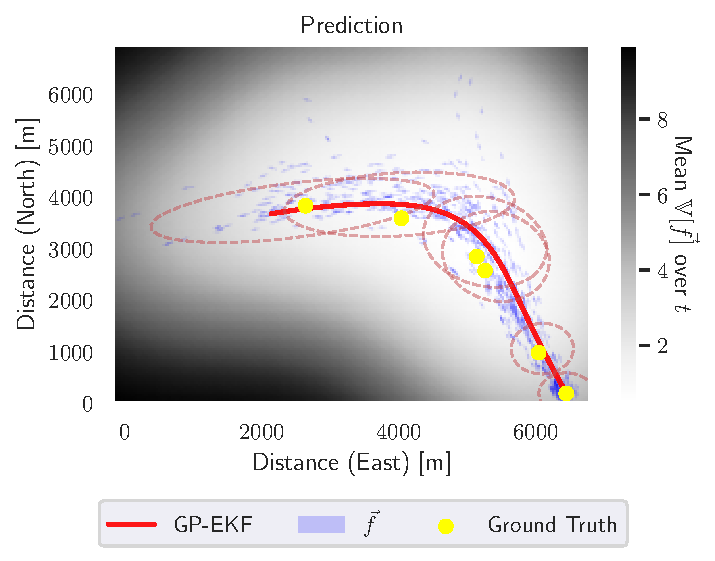
\includegraphics[width=\textwidth]{figures/dyngp/gp_ekf.pdf}
        \caption{Trajectory plotted against the vector-field $\vec{f}(\boldsymbol{x})$. The ellipses show the $95\%$ credibility interval for the predicted trajectory at the ground-truth timestamps.}
    \end{subfigure}
    \begin{subfigure}{\textwidth}
        \centering
        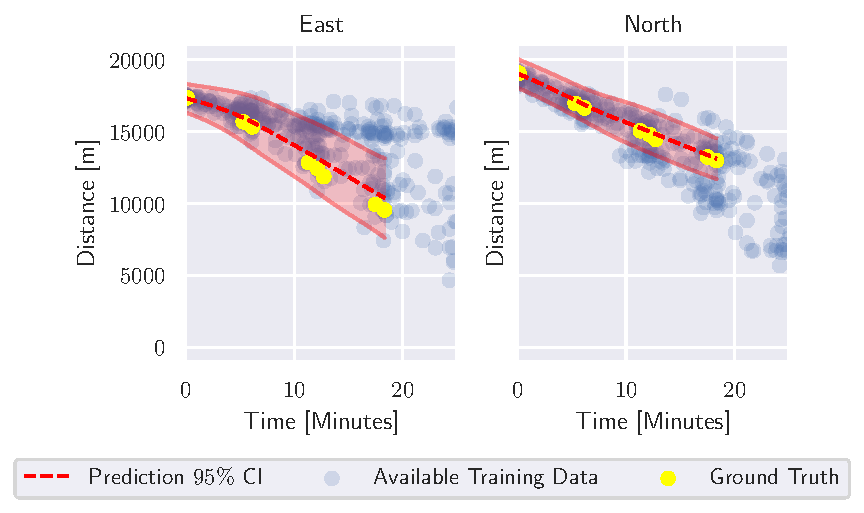
\includegraphics[width=\textwidth]{figures/dyngp/gp_ekf_state.pdf}
        \caption{$95\%$ credibility interval for the trajectory plotted against time}
    \end{subfigure}
    \caption{Predicted position using GP-EKF}
    \label{fig:gp_ekf}
\end{figure}



\section{Incorporating vessel position}
While the prediction procedure proposed in \cref{alg:gp_ekf_prediction} yields good predictions in many cases, it is inherently an open-loop prediction. Inaccurate predictions will never be corrected, propagating through any remaining iterations, potentially leading to significant errors later on. \todo[]{Add figure to showcase this issue} It would be desirable if the prediction converged towards available position measurements, \textit{slowly and only if the prediction is clearly wrong}. In other words, weak feedback compensating for minor prediction errors. Expressed using Bayes law
\begin{equation}\label{eq:gp_ekf_update_posterior}
    p(\boldsymbol{x}_{0:t} | \mathcal{D}) = \frac{p(\mathcal{D} | \boldsymbol{x}_{0:t}) p(\boldsymbol{x}_{0:t})}{p(\mathcal{D})} \propto p(\mathcal{D} | \boldsymbol{x}_{0:t})p(\boldsymbol{x}_{0:t})
\end{equation}
where $\mathcal{D}$ here is all available training data.

The problem is that the dataset $\mathcal{D}$ does not contain any samples from the target vessel's future trajectory, though it contains a lot of data from trajectories that are assumed to be similar. Thus, the challenge is to relate the target vessel's trajectory to the data-generating process for the dataset $\mathcal{D}$.

This is still very much considered an unsolved problem. This thesis attempts two different approaches, but the solutions are not yet satisfactory.

\subsection{Synthetic Likelihood}
This section is inspired by the work of \citeauthor{praveen-syn} \cite{praveen-syn}.

A proper likelihood $p(\mathcal{D} | \boldsymbol{x}_{0:t})$ is unavailable, or at least considered infeasible to compute. This motivates the use of so-called \textit{likelihood-free} methods, where the most common method is the \textit{Approximate Bayesian Computation} (ABC). Likelihood-free methods are used when the likelihood cannot be computed, while simulation from the model is still possible \cite{likelihood_free,frazier2021bayesian}. In this thesis, the focus will be on another likelihood-free approach, namely, the \textit{\acrfull{sl}} which replaces the likelihood by one or several approximate Gaussian summary statistics, $S_{0:t} = S(\boldsymbol{x}_{0:t}) \sim \mathcal{N}(\boldsymbol{\mu}(\boldsymbol{x}_{0:t}), \boldsymbol{\Sigma}(\boldsymbol{x}_{0:t}))$, of the data. Assuming the summary statistic contains sufficient information about $\boldsymbol{x}_{0:t}$, it should yield a good approximation of the true likelihood, i.e.
\begin{equation}
    p(\mathcal{D} | \boldsymbol{x}_{0:t}) \approx p(S_{0:t} | \boldsymbol{x}_{0:t})
\end{equation}

In this thesis, the likelihood is assumed to factorize into
\begin{equation}
    p(S_{0:T} | \boldsymbol{x}_{0:T}) = \prod_{t=0}^{T} p(S_t | \boldsymbol{x}_t)
\end{equation} and the summary statistic $S_i$ is selected as the mean of the samples in the vicinity of $\boldsymbol{x}_i$. A simple solution is to define the vicinity as a fixed radius around the state $\boldsymbol{x}_i$

\begin{equation}
    \mathcal{Y}_t = \mathcal{Y}_t(\boldsymbol{x}_t) = \{\boldsymbol{z}_i \in \mathcal{D} : \; ||\boldsymbol{x}_t - \boldsymbol{z}_i|| \leq r\}
\end{equation}
where the threshold $r$ is a fixed parameter. The summary statistic $S_i$ is then given by

\begin{equation}
    S_t = S(\boldsymbol{x}_t) = \frac{1}{N} \sum_{\boldsymbol{z}_i \in \mathcal{Y}_t} \boldsymbol{z}_i
\end{equation}
where $N$ is the number of samples in $\mathcal{Y}_t$. Assuming a simple measurement model
\begin{equation}\label{eq:gp_ekf_sl_z}
    \boldsymbol{z} = \boldsymbol{x} + \epsilon, \quad \epsilon \sim \mathcal{N}(0, \boldsymbol{R})
\end{equation}

which yields the following distribution for the summary statistic given the predicted state $\boldsymbol{x}_i$.

\begin{equation}
    p(S_t \;| \; \boldsymbol{x}_t) = \mathcal{N}(\boldsymbol{x}_t, \frac{\boldsymbol{R}}{N})
\end{equation}

The posterior distribution of the trajectory prediction can then be approximated by

\begin{align}\label{eq:gp_ekf_sl_approx_posterior}
    \begin{split}
        p(\boldsymbol{x}_{0:t} | \mathcal{D}) \approx p(\boldsymbol{x}_{0:t} | S_{0:t}) &= \frac{p(S_{0:t} | \boldsymbol{x}_{0:t}) p(\boldsymbol{x}_{0:t})}{p(S_{0:t})}\\
        &= \frac{p(S_t | \boldsymbol{x}_t)p(\boldsymbol{x}_t | \boldsymbol{x}_{t-1}) p(\boldsymbol{x}_{0:t-1} | S_{0:t-1})}{p(S_t | S_{0:t-1})}
    \end{split}
\end{align}
where the second equality yields a recursive formulation for the posterior distribution. As all distributions are Gaussian, \cref{eq:gp_ekf_sl_approx_posterior} boils down to the normal Kalman update step, using the summary statistic $S_i$ as measurement for each timestep.

The derivations in this section blindly make quite substantial assumptions that can seriously impact the results.
\begin{enumerate}
    \item The derivations claim the summary statistics are approximate Gaussian by the central limit theorem. The underlying assumption is that the data is \acrshort{iid} and that there is a large number of samples. As the samples originate from several types of vessels and from different trajectories, there is reason to suspect the samples might not be \acrshort{iid}.
    \item The measurement model in \cref{eq:gp_ekf_sl_z} assumes the measurements are distributed around the target vessel's trajectory. In practice, the samples might be heavily influenced by several different trajectories at once. This makes tuning $\boldsymbol{R}$ a challenge.
\end{enumerate}


\begin{figure}
    \centering
    \begin{subfigure}{\textwidth}
        \centering
        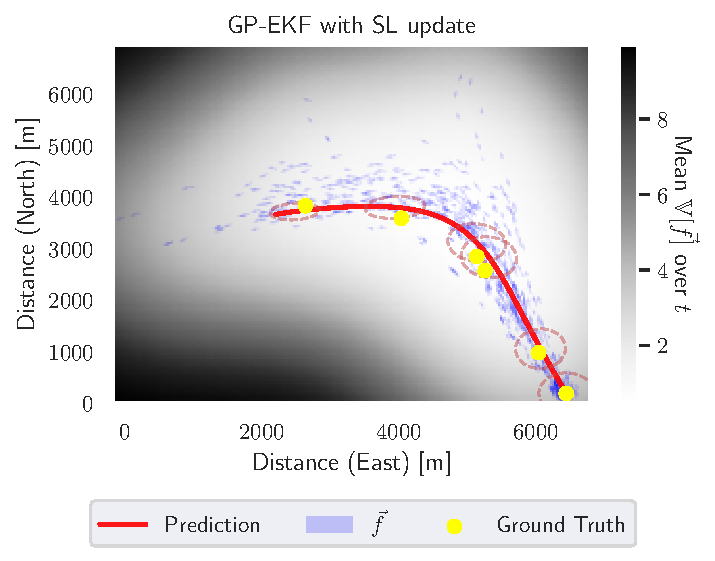
\includegraphics[width=\textwidth]{figures/dyngp/gp_ekf_with_syn.pdf}
        \caption{Trajectory plotted against the vector-field $\vec{f}(\boldsymbol{x})$. The ellipses show the $95\%$ credibility interval for the predicted trajectory at the ground-truth timestamps.}
    \end{subfigure}
    \begin{subfigure}{\textwidth}
        \centering
        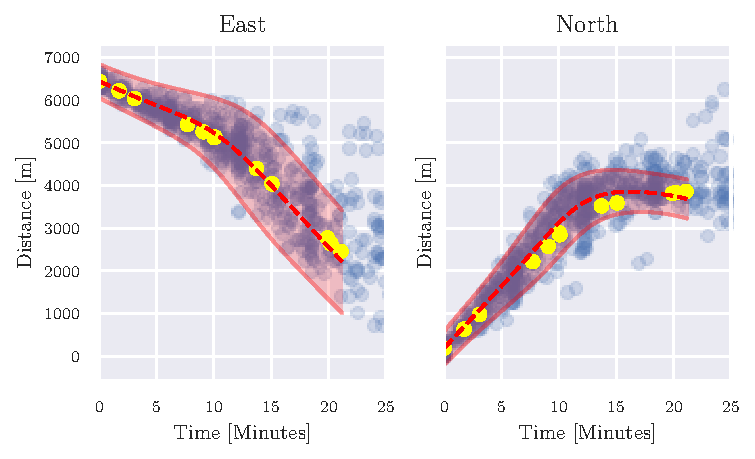
\includegraphics[width=\textwidth]{figures/dyngp/gp_ekf_with_syn_state.pdf}
        \caption{$95\%$ credibility interval for the trajectory plotted against time}
    \end{subfigure}
    \caption{Predicted position with the \acrshort{sl} update procedure.}
    \label{fig:gp_ekf_with_syn}
\end{figure}


\subsection{Probabilistic Data Association Filter}
The \acrshort{sl} update above ends up using an overly simplistic measurement model and does not consider the possibility that some measurements may originate from different underlying trajectories. For the target vessel following a specific underlying trajectory, the dataset may actually contain substantial false measurements which negatively affect the prediction. As the \acrshort{sl} update has no notion of false measurements, the result is overconfident uncertainty measurements can be seen in \cref{fig:gp_ekf_with_syn}.

This section attempts a rather different approach by incorporating the notion of data association into the mix. More specifically, the idea is to view the entire problem as single-target tracking and then apply the \textit{\acrfull{pdaf}} to solve the problem.

The \acrshort{pdaf} is a method commonly used in target tracking which combines data association and filtering. The following introduction to \acrshort{pdaf} is mostly inspired by \cite{sensorfusjon}, with some adaptations to fit the current problem better. As single target tracking and data association is not the topic of this thesis, only a short introduction to the \acrshort{pdaf} will be included here. For more details, see \cite{sensorfusjon,bar1995multitarget}

In this section, all measurements in the available training set are considered as \textit{virtual} \footnote{Virtual meaning a measurement that did not originate from the target vessel, but rather a measurement that could potentially originate from the target in the future. The word measurement is still used to keep the terminology similar to what is used by \acrshort{pdaf}.} position measurements, which may or may not originate from the vessel at time $t$. It is assumed \textbf{at most one} measurement may originate from the target to reduce the computational complexity significantly \cite{sensorfusjon}. The rest of the measurements are assumed to be clutter.

Given the predicted state $\hat{\boldsymbol{x}}_t$, any real measurement is expected to be distributed around this state due to some measurement noise. Following the notation used by \acrshort{ekf}, and using the measurement model $h(\boldsymbol{x}) = \boldsymbol{x} \implies H = \frac{\partial h (\boldsymbol{x})}{\partial \boldsymbol{x}} = I$, the predicted measurement distribution is expressed as in \cref{eq:gp_ekf_pdaf_measurement} where the innovation covariance is defined as $\boldsymbol{S}_t \triangleq \hat{\boldsymbol{P}}_t + \boldsymbol{R}$ and $\boldsymbol{R}$ is the measurement noise.

\begin{equation} \label{eq:gp_ekf_pdaf_measurement}
    \hat{\boldsymbol{z}}_t \sim \mathcal{N}(\hat{\boldsymbol{x}}_t, \boldsymbol{S}_{t}) = \mathcal{N}(\hat{\boldsymbol{x}}_t, \hat{\boldsymbol{P}}_t + \boldsymbol{R})
\end{equation}

There is also the possibility that none of the measurements originated from the target, and all observations are clutter. A good clutter model is a complicated topic, but the Poisson clutter model is used in this thesis. As the measurements are not actual measurements from the target, it is difficult to assign meaning to any clutter model. It, therefore, simply boils down to which parameters need to be tuned \footnote{The trajectory prediction is here considered to be target tracking of future position. The clutter parameters, therefore, need to be interpreted in the context of target tracking, not trajectory prediction.} and the Poisson clutter model should already be familiar to anyone with experience in target tracking.
Using the Poisson clutter model, the association probabilities are given by \cref{eq:pdaf_clutter_association_prob} \cite{sensorfusjon}, where $a_t$ is a discrete variable following a Categorical distribution where $a_t=k > 0$ denotes that measurement $k$ originated from the target. $a_t = 0$ is the special case when none of the measurements originated from the target, i.e., the predicted state should not be updated. $Z$ denotes a matrix of all the measurements (positions) available in the training data and is independent of time, i.e., all measurements are always potential candidates. $\lambda$ denotes the clutter rate, and $P_D$ denotes the probability of detecting the target vessel.
\begin{equation}\label{eq:pdaf_clutter_association_prob}
    \Pr\{a_t | Z\} \propto \begin{cases}
        \lambda (1 - P_D)                                                                 & a_t = 0 \\
        P_D \mathcal{N} (\boldsymbol{z}^{a_t} | \hat{\boldsymbol{x}}_t, \boldsymbol{S}_t) & a_t > 0 \\
    \end{cases}
\end{equation}

Using the likelihood for each of the possible outcomes, the association probabilities $\boldsymbol{\beta}$ can be computed by normalizing the likelihood, i.e.

\begin{equation}
    \beta_t^{a_t=i} = \frac{\Pr\{a_t=i \; | \; Z\}}{\sum_{k=0}^M \Pr\{a_t=k \; | \; Z\}}
\end{equation}

The predicted state can then by updated using the Kalman update procedure for each the measurements individually. As the measurements $\boldsymbol{z}_t^{a_t > 0}$ are known values, the state innovation $\boldsymbol{v}_t^{a_t>0} \triangleq \boldsymbol{z}_t^{a_t>0} - \hat{\boldsymbol{z}}_t$ is distributed according to the measurement prediction $\hat{\boldsymbol{z}}_t$.

\begin{equation}
    \boldsymbol{v}_t^{a_t>0} \sim \mathcal{N}(\boldsymbol{z}_t^{a_t>0} - \hat{\boldsymbol{x}}_t, S_t)
\end{equation}
The updated state for each measurement is then given by the normal \acrshort{ekf} update step

\begin{subequations}
    \begin{align}
        \boldsymbol{x}_t^{a_t > 0} & = \hat{\boldsymbol{x}}_t + \boldsymbol{W}_t \boldsymbol{v}_t^{a_t > 0} \\
        \boldsymbol{P}_t^{a_t > 0} & = \ (\boldsymbol{I} - \boldsymbol{W}_t) \hat{\boldsymbol{P}}_t
    \end{align}
\end{subequations}
where $\boldsymbol{W}_t \triangleq \hat{\boldsymbol{P}}_t \boldsymbol{S}_t^{-1}$ is the Kalman gain.
The updated state of the vessel over all possible measurements can be described as a Gaussian Mixture Model over the $M+1$ different modes weighted by the association probabilites, i.e.
\begin{equation}
    p(\boldsymbol{x_t}) = \underbrace{\beta_t^{a_t=0} \mathcal{N}(\boldsymbol{x}_t \; | \; \hat{\boldsymbol{x}}_t, \hat{\boldsymbol{P}}_t)}_{\text{No measurements are valid}} + \sum_{k=1}^M \underbrace{\beta_t^{a_t=k} \mathcal{N}\big(\boldsymbol{x}_t | \boldsymbol{x}_t^{a_t=k}, \boldsymbol{P}_t^{a_t=k}\big)}_{\text{Measurement $k$ is valid}}
\end{equation}


Moment reduction is then used to combined the different hypothesises into a single unimodal Gaussian distribution, i.e. a Gaussian distribution is fitted to the first and second moment (mean and variance) of the Gaussian mixture. The mean and variance of the resulting distribution is given by \cref{eq:pdaf_moment_mean} and \cref{eq:pdaf_moment_var} respectively, using $\boldsymbol{v}_t \triangleq \sum_{a_t > 0} \beta_t^{a_t} \boldsymbol{v}_t^{a_t}$.

\begin{subequations}
    \begin{align}
        \boldsymbol{x}_t & = \hat{\boldsymbol{x}}_t + \boldsymbol{W}_t \boldsymbol{v}_t \label{eq:pdaf_moment_mean} \\
        \begin{split}
            \boldsymbol{P}_t &= \hat{\boldsymbol{P}}_t - (1 - \beta_t^{0}) \boldsymbol{W}_t \boldsymbol{S}_t  \boldsymbol{W}_t\\ &+ \underbrace{\boldsymbol{W}_t \big[\sum_{a_t > 0}^M \beta_t^{a_t} \boldsymbol{v}_t^{a_t} (\boldsymbol{v}_t^{a_t})^\intercal - \boldsymbol{v}_t \boldsymbol{v}_t^\intercal \big] \boldsymbol{W}_t^\intercal}_{\text{spread of innovation}}\label{eq:pdaf_moment_var}
        \end{split}
    \end{align}
\end{subequations}

While available measurement could be used at each timestep, it is in practice more convenient only to include a subset that is close enough to the predicted state. As this measurement \textit{gate} should scale with the uncertainty, the gated subset is selected as \cref{eq:pdaf_gate} where $g$ is the number of standard deviations the method should consider.

\begin{equation} \label{eq:pdaf_gate}
    \mathcal{G} = \big\{ \boldsymbol{z}^{a_t > 0} \; | \; (\boldsymbol{z}^{a_t > 0} - \hat{\boldsymbol{x}}_t)^\intercal S^{-1} (\boldsymbol{z}^{a_t > 0} - \hat{\boldsymbol{x}}_t) < g^2 \big\}
\end{equation}


By combining the \acrshort{pdaf} update with the GP-EKF prediction procedure in \cref{alg:gp_ekf_prediction}, the predicted trajectory can be tuned to favor areas with a large number of samples, effectively pulling the state towards areas with available samples. Conversely, in regions with samples spread evenly around the predicted state, then the \acrshort{pdaf}'s effect is negligible (assuming proper tuning). 

\begin{algorithm}[h]
    \begin{algorithmic}[1]
        \Procedure{GP-EKF-PDAF}{$\hat{\boldsymbol{x}}_{t}$, $\hat{\boldsymbol{P}}_{t}$, | $\mathbf{R}$, $\lambda$, $p_D$, $g$}
        \State $\boldsymbol{S}_t = \hat{\boldsymbol{P}}_t + \boldsymbol{R}$ \Comment{Innovation Covariance}
        \State $\boldsymbol{W}_t = \hat{\boldsymbol{P}}_t \boldsymbol{S}_t^{-1}$\Comment{Kalman Gain}
        \For{each measurement $\boldsymbol{z}^{a_t > 0}$}
        \State $\boldsymbol{v}_t^{a_t>0} = \boldsymbol{z}^{a_t>0} - \hat{\boldsymbol{x}}_t$ \Comment{Innovation}
        \State $\tilde{\beta}^{a_t>0} = \mathcal{N}(\boldsymbol{v}_t^{a_t > 0} \; | \; 0, \boldsymbol{S}_t)$ \Comment{Unnormalized Weight}
        \EndFor
        \State $\tilde{\beta}_t^{a_t = 0} = \lambda (1-p_D)$ \Comment{Unnormalized Clutter Probability}
        \State $\boldsymbol{\beta} = \frac{\tilde{\boldsymbol{\beta}}}{\sum_{a_t} \tilde{\beta}^{a_t}}$ \Comment{Normalize weights}
        \State $\boldsymbol{v}_t = \sum_{a_t > 0} \beta^{a_t} \boldsymbol{v}_t^{a_t}$
        \State $\boldsymbol{x}_t = \hat{\boldsymbol{x}}_t + \boldsymbol{W}_t \boldsymbol{v}_t$\Comment{Update the state mean}
        \State $\tilde{\boldsymbol{P}}_t = \boldsymbol{W}_t \big[\sum_{a_t > 0}^M \beta_t^{a_t} \boldsymbol{v}_t^{a_t} (\boldsymbol{v}_t^{a_t})^\intercal - \boldsymbol{v}_t \boldsymbol{v}_t^\intercal \big] \boldsymbol{W}_t^\intercal$\Comment{Spread of innovation}
        \State $\boldsymbol{P}_t = \hat{\boldsymbol{P}}_t - (1 - \beta_t^{0}) \boldsymbol{W}_t \boldsymbol{S}_t  \boldsymbol{W}_t + \tilde{\boldsymbol{P}}_t$ \Comment{Updated state uncertianty}


        \State \textbf{return} $\boldsymbol{x}_t, \; \boldsymbol{P}_t$
        \EndProcedure
    \end{algorithmic}
    \caption{GP-EKF-PDAF update}
    \label{alg:gp_ekf_pdaf}
\end{algorithm}


\begin{figure}
    \centering
    \begin{subfigure}{\textwidth}
        \centering
        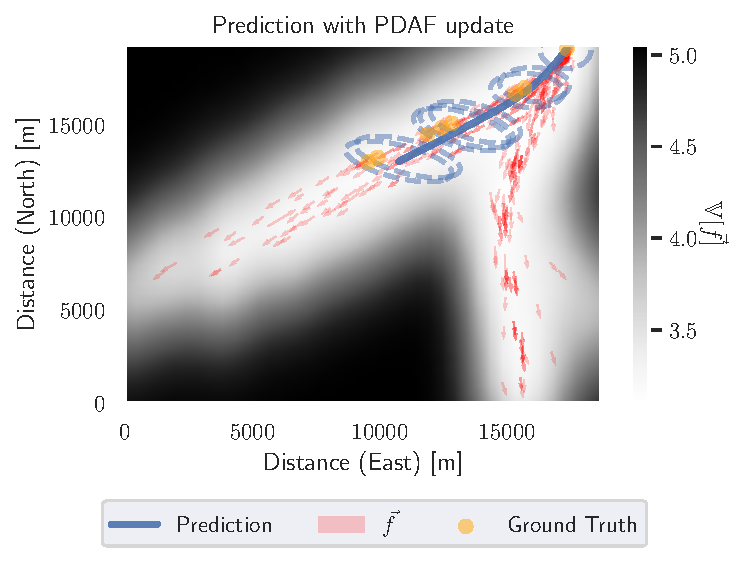
\includegraphics[width=\textwidth]{figures/dyngp/gp_ekf_with_pdaf.pdf}
        \caption{Trajectory plotted against the vector-field $\vec{f}(\boldsymbol{x})$. The ellipses show the $95\%$ credibility interval for the predicted trajectory at the ground-truth timestamps.}
    \end{subfigure}
    \begin{subfigure}{\textwidth}
        \centering
        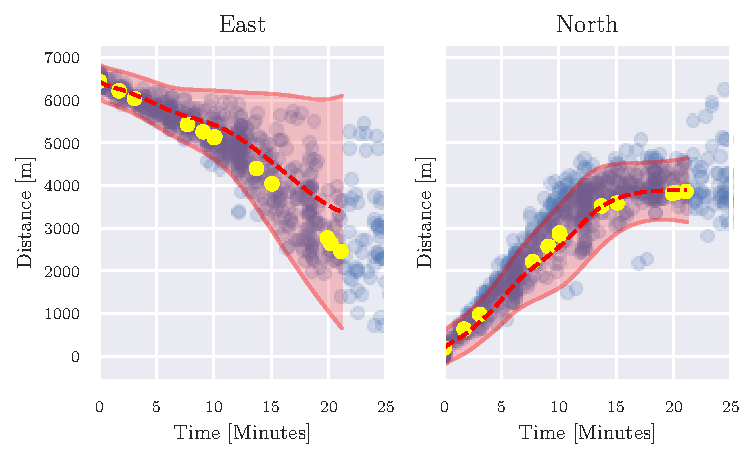
\includegraphics[width=\textwidth]{figures/dyngp/gp_ekf_with_pdaf_state.pdf}
        \caption{$95\%$ credibility interval for the trajectory plotted against time}
    \end{subfigure}
    \caption{Predicted position with the PDAF update procedure.}
    \label{fig:gp_ekf_with_pdaf}
\end{figure}

\subsubsection{Tuning PDAF parameters}
The model should primarily trust the prediction model, as it would get stuck as the measurements do not change over time. If the \acrshort{pdaf} parameters are tuned too aggressively, it tends to affect the velocity estimates of the prediction negatively. In practice, it has worked well tuning the measurement noise $\boldsymbol{R}$ to get the desired update effect.
However, finding a set of parameters that works well across different trajectories turns out to be challenging. Parameters that improve the prediction for one trajectory may do more harm than good on another. The performance of using PDAF will be explored further in \cref{chap:stat_testing}.

% \subsection{The ad-hoc approach}\todo[]{Consider removing}
% Neither the \acrshort{sl} nor the \acrshort{pdaf} approach is a satisfactory solution as both either have a negligible effect or suffers from overconfident uncertainty predictions. The problem lies in the assumptions that the observed positions originate from the target vessel, while in reality, the measurements are from entirely different trajectories. As long as the predicted state is in a densely populated area, the update steps will have no problem finding evidence supporting the current state, leading to overconfidence. Though not covered in this thesis, this problem motivates research into more sophisticated likelihood functions.

% During tuning both these methods, it became apparent that the desired behavior of these update steps would correct the prediction's mean and keep roughly the same level of uncertainty. In other words, the model should use the additional information from the update step to correct its prediction without reducing the uncertainty. While certainly not elegant, the quick and dirty solution was to omit the update of the state uncertainty, i.e., $\boldsymbol{P}_t = \hat{\boldsymbol{P}}_t$. This ad-hoc solution will be denoted the \textit{modified \acrshort{pdaf}} and the \textit{modified \acrshort{sl}} and works surprisingly well in practice. It is, however, not considered a good replacement for a proper likelihood.

\subsection{Simulating trajectories using Gaussian Process Sequential Monte Carlo}\label{sec:dyngp_particle}
The Kalman-based prediction scheme proposed in the previous section works well as long as a single Gaussian distribution can sufficiently explain the uncertainty. However, in branching trajectories, minor differences in position early in the predicted trajectory might significantly affect the following predictions. The result is a multimodal trajectory distribution, which a Kalman-based approach is not able to express.

Inspired by the prediction step used by \textit{particle filters} \cite{sensorfusjon}, the idea of sampling trajectories can be used to explore the multimodal trajectory distribution. While inspired by the particle filter, this approach will from now on be referred to as \textit{Sequential Monte-Carlo} to avoid confusion\footnote{a vital part of the particle filter is weighting the particles based on available measurements. As only the sampling of trajectories is performed, Sequential Monte-Carlo seems like a better fit.}, as well as to follow the same naming convention as used by \citeauthor{pedestrian} \cite{pedestrian}.

The derivation of the Sequential Monte-Carlo approach is embarrassingly simple as this method trades high computational complexity for more straightforward mathematics. Instead of analytical propagation of uncertainty, many trajectories are simulated through random sampling and used to express the uncertainty empirically. As a result, the uncertainty for any trajectory distribution can be described, though at the cost of considerable computational complexity.
$N$ different trajectories are initialized with similar initial conditions. The trajectories are then simulated by drawing independent increments from $\vec{f}$ using the approach described in \cref{sec:gp_samples}, conditioned on the current state of each trajectory. The result is visualized in \cref{fig:gp_particle} for $N=500$ trajectories.
\begin{figure}[h]
    \centering
    %\begin{subfigure}{\textwidth}
    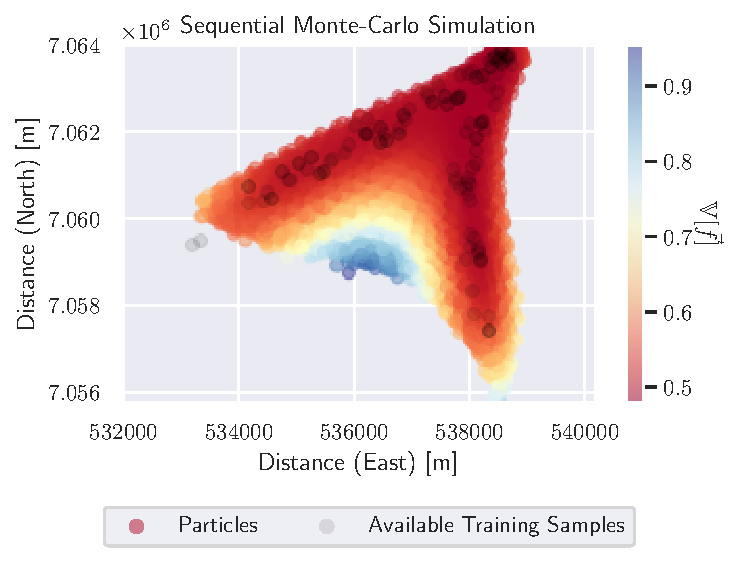
\includegraphics[width=\textwidth]{figures/dyngp/gp_particle.pdf}
    \caption{Trajectories simulated by sampling from $\vec{f}$. Notice how it is able to represent the multimodal trajectory distribution. }
    %\end{subfigure}
    %\begin{subfigure}{\textwidth}
    %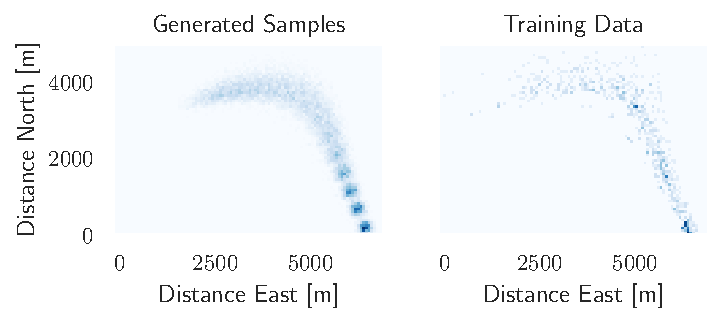
\includegraphics[width=\textwidth]{figures/gp_particle_hist.pdf}
    %\caption{}
    %\end{subfigure}
    \label{fig:gp_particle}
\end{figure}

\subsection{Training Source}
There are two potential sources for the training samples $\boldsymbol{y}$:

\begin{enumerate}
    \item Trajectories from the dataset are converted into training samples for $\vec{f}$ using the simple first-order finite-difference method in \cref{eq:finite_difference} between subsequent \acrshort{ais} samples in a trajectory $i$. This yields the training outputs $\boldsymbol{y}_t^{i}$ corresponding to the inputs $\boldsymbol{\eta}_t^i$ such that $\boldsymbol{y}_t^i = \vec{f}(\boldsymbol{\eta}_t^i) + \epsilon$.
    \item The \acrshort{cog} and \acrshort{cog} from the \acrshort{ais} data can be used directly.
\end{enumerate}

\begin{align}\label{eq:finite_difference}
    \boldsymbol{y}_t = \frac{\boldsymbol{x}_{t+1} - \boldsymbol{x}_t}{\tau_{t+1} - \tau_t}
\end{align}

A concern with using the \acrshort{cog} and \acrshort{sog} from the \acrshort{ais} is that this assumes the vessel's own estimates are accurate. The effect of this design choice is investigated further in \cref{chap:stat_testing}.


\section{Choice of kernel}
The approximation used to calculate the posterior distribution in \cref{eq:dyngp_true_posterior} is only a first-order Taylor approximation. Hence, it is only a reasonable approximation for functions with a low degree of nonlinearity, and care should be taken when designing the \acrshort{gp} dynamics $\vec{f}$. In this thesis, it is argued that \acrshort{rbf} kernel is the preferred choice due to the highly smooth characteristic of the functions drawn from this kernel. The \acrshort{rbf} kernel

\begin{equation}\label{eq:dyngp_kernel}
    k(\boldsymbol{\eta}, \boldsymbol{\eta}') = \sigma^2 \exp \big[ - \frac{1}{2} (\boldsymbol{\eta} - \boldsymbol{\eta}')^\intercal \boldsymbol{W}^{-1} (\boldsymbol{\eta} - \boldsymbol{\eta}')^\intercal\big]
\end{equation}
is found to work well in most cases, as long as the vessel follows a reasonably smooth trajectory. $\boldsymbol{W}$ is a diagonal matrix a separate lengthscale for each input dimension. The \acrshort{rbf} is the go-to kernel for the GP-EKF in this thesis, though other kernels, such as the Matern class of kernels, may work just as well, if not better.

The derivative of this kernel with respect to the $i$-th input dimension $\boldsymbol{\eta}[i]$ can be computed as

\begin{equation}
    \frac{\partial k(\boldsymbol{\eta}, \boldsymbol{\eta}')}{\partial \boldsymbol{\eta}[i]} = -W_{ii}^{-1}(\boldsymbol{\eta}[i] - \boldsymbol{\eta}'[i]) \sigma^2 \exp \big[ - \frac{1}{2} (\boldsymbol{\eta} - \boldsymbol{\eta}')^\intercal \boldsymbol{W}^{-1} (\boldsymbol{\eta} - \boldsymbol{\eta}')^\intercal\big]
\end{equation}


A possible extension is to use the sum of two \acrshort{rbf} kernels to get some additional flexibility while still having a reasonably smooth function. This is the same kernel proposed in \cref{chap:direct_gp}, though without the \acrshort{cog} and \acrshort{sog} input dimensions. It works better than the \acrshort{rbf} kernel in some of the more complicated cases, though at the cost of more hyperparameters to tune. In simple cases, hyperparameter optimization \textbf{typically} reduces the scale parameter of one of the \acrshort{rbf} kernels such that the dependent noise kernel $k_1$ has a negligible effect. It is important to stress the word "typically," as this kernel is also more prone to bad local optima during hyperparameter optimization due to the additional parameters \cite{rasmussen} and may end up overfitting. If the length scales become too small, the dynamics $\vec{f}$ is allowed to become highly non-linear, and small changes in the input $\boldsymbol{x}$ may have a large impact on the prediction. The Taylor approximation is not a reasonable approximation in these cases, and the result is unstable uncertainty estimates \footnote{This is typically seen in the uncertainty estimates as large steps at seemingly random time steps, where the uncertainty experience sudden jumps as some elements in the Jacobian become large.}. The key takeaway is that the more flexible kernels are also more prone to overfitting, and care should be taken during optimization to avoid unrealistic parameters.

Other kernels may be preferred if the posterior density in \cref{eq:dyngp_true_posterior} is evaluated using sampling-based methods, such as Sequential Monte-Carlo, as the Taylor approximation does not limit these methods.  However, it is not covered by this thesis.


\subsection{Optimizing the hyperparameters}
The hyperparameters can be optimized using the \acrshort{ml} approach discussed in \cref{sec:gp_mle}.

The whole dataset cannot be used to find the optimal hyperparameters due to the computational complexity. Two approaches are proposed to mitigate this issue:
\begin{enumerate}
    \item Fit the hyperparameter to many different subsets of the available training data and use the median values. The median is preferred over the mean values to avoid issues with outlier parameter estimates. This approach tends to find a set of hyperparameters that work well across a wide range of cases but may become too general for challenging scenarios.
    \item Rerun the hyperparameter optimization for each scenario. This approach tends to find the optimal parameters in each case. However, it is also error-prone as it is not guaranteed to find a global optimum, and it may cause overfitting.
\end{enumerate}

The first approach is likely the preferred choice in practical applications, as the hyperparameter optimization is prone to bad local optima, and the results should ideally be inspected before deployment to real-world applications. A possible extension is to find a global set of parameters for each distinct vessel type, assuming a vessel's behavior is somewhat consistent across the entire region.

\section{Summary}
This chapter has so far introduced a lot of new concepts so that it might be nice with a summary of the overall pipeline:

\begin{enumerate}
    \item Based on the target vessel's current state, such as position, \acrshort{cog} and \acrshort{sog}, trajectories with similar initial conditions is selected from the training set.
    \item Training inputs $\boldsymbol{\eta}$ and outputs $\boldsymbol{y}$ for $\vec{f}$ are generated from the training trajectories.
    \item The kernel hyperparameters are optimized using \acrshort{ml} to find the parameters which best explains the training data. This is either done once to find a global set of parameters or individually for each scenario.
    \item The training data and kernel can then used to get the conditional distribution for $\vec{f}$.
    \item The \acrshort{ekf} procedure in \cref{alg:gp_ekf_prediction} is called repeatedly, using the current state of the target vessel as initial conditions. At each step, the \acrshort{pdaf} update procedure can be used as well if desired. Sequential Monte-Carlo can alternatively be used to simulate multimodal trajectories.
\end{enumerate}

The only parameters which need manual tuning are the time increment $\Delta \tau$ and the initial covariance $\boldsymbol{P}_0$. All other parameters are learned from the data.
